\documentclass{article}
\usepackage{graphicx,subcaption,lineno}
\usepackage{amsmath, amsthm, amsfonts, amssymb}
\usepackage{multirow,microtype}
\usepackage{longtable}

\frenchspacing

\renewcommand{\thefigure}{S\arabic{figure}}
\renewcommand{\thetable}{S\arabic{table}}

\setcounter{figure}{0}
\setcounter{table}{0}

\title{Supplemental information for ``Death and taxa''}
\author{Peter D Smits}
\date{}

\begin{document}
\maketitle

\section{Supertree inference}
As there is no single, combined formal phylogenetic hypothesis of all Cenozoic fossils mammals from North America, it was necessary to construct a semi-formal supertree. This was done by combining taxonomic information for all the observed species and a few published phylogenies. 

The initial taxonomic classification of the observed species was based on the associated taxonomic information from the PBDB. This information was then updated using the Encyclopedia of Life (http://eol.org/) which collects and collates taxonomic information in a single database. This was done programatically using the \texttt{taxize} package for R \cite{2013taxize}. Finally, this taxonomic information was further updated using a published taxonomy of fossil mammals \cite{Janis1998,Janis2008}. 

This taxonomy serves as an initial phylogenetic hypothesis which was then combined with a selection of species-level phylogenies \cite{Bininda-Emonds2007,Raia2012f} in order to better constrain a minimum estimate of the actual phylogenetic relationships of the species. The supertree was inferred via matrix representation parsimony implemented in the \texttt{phytools} package for R \cite{revell2012phytools}. Of the two most parsimonious trees found, I used only one for analysis.

Polytomies were resolved in order of species first appearance in order to minize stratigraphic gaps. The resulting tree was then time scaled using the \texttt{paleotree} package via the ``minimum branch length'' approach with a minimum length of 0.1 My \cite{Bapst2012a}. The minimum length is necessary to avoid zero-length branches which cause the phylogenetic covariance matrix not to be positive definite, which is important for computation (see below). While other time scaling approaches are possible \cite{Hedman2010,Bapst2013a} this method was chosen for its simplicity and not requiring additional information about diversification rates which are the interest of this study.

\section{Modeling censored observations}
Censored data are modeled using the survival function of the distribution, \(S(t)\), defined earlier for the Weibull distribution (Eq. 5, 6) with \(\sigma\) defined as above (Eq. 8, 9). \(S(t)\) is the probability that an observation will survive longer than a given time \(t\). 

The likelihood of uncensored observations is evaluated as normal using equation 4 while right censored observations are evaluated at \(S(t)\) and left censored observations are evaluated at \(1 - S(t)\). Note, \(1 - S(t)\) is equivalent to the cumulative distribution function and \(S(t)\) is equivalent to the complementary cumulative distribution function \cite{Gelman2013d}.

The final sampling statement/likelihood for both uncensored and both right and left censored observations is then written
\begin{equation*}
  L \propto \prod_{i \in C} \mathrm{Weibull}(y_{i} | \alpha, \sigma) \prod_{j \in R} S(y_j | \alpha, \sigma) \prod_{k \in L} \left(1 - S(y_{k} | \alpha, \sigma)\right),
\end{equation*}
where \(C\) is the set of uncensored observations, \(R\) is the set of right censored observations, and \(L\) is the set of left censored observations.

\section{Deviance residuals}
% need a few definitions from the main text
In standard linear regression, residuals are defined as \(r_{i} = y_{i} - y_{i}^{est}\). For the model used here, this definition is inadequate. The equivalent values for survival analysis are deviance residuals. To define how deviance residuals are calculated, we first define the cumulative hazard function \cite{Klein2003}. Given \(S(t)\), we define the cumulative hazard function as 
\begin{equation*}
  \Lambda(t) = -log\left(S\left(t\right)\right).
\end{equation*}

Next, we define martingale residuals \(m\) as
\begin{equation*}
  m_{i} = I_{i} - \Lambda(t_i).
\end{equation*}
\(I\) is the inclusion vector of length \(n\), where \(I_{i} = 1\) means the observation is completely observed and \(I_{i} = 0\) means the observation is censored. Martingale residuals have a mean of 0, range between 1 and \(-\infty\), and can be viewed as the difference between the observed number of deaths between 0 and \(t_{i}\) and the expected number of deaths based on the model. However, martingale residuals are asymmetrically distributed, and can not be interpreted in the same manner as standard residuals. 

The solution to this is to use the deviance residuals, \(D\). This is defined as a function of martingale residuals and takes the form
\begin{equation*}
  D_{i} = \text{sign}(m_{i}) \sqrt{-2[m_{i} + I_{i}log(I_{i} - m_{i})]}.
\end{equation*}
Deviance residuals have a mean of 0 and a standard deviation of 1 by definition.

\section{Variance partitioning}
I calculated VPC using a resampling approach based on \cite{Goldstein2002}. The procedure is as follows:
\begin{enumerate}
  \item Simulate \(w\) (50,000) values of \(\eta\); \(\eta \sim \mathcal{N}(0, \sigma_{c})\).
  \item For a given value of \(\beta^{T} \mathbf{X}\), calculate \(\sigma^{c*}\) (Eq. 7) for all \(w\) simulations, holding \(h\) constant at 0.
  \item Calculate \(\upsilon_{c}\), the Weibull variance (Eq.~\ref{eq:wei_var}) of each element of \(\sigma^{c*}\) with \(\alpha\) drawn from the posterior estimate.
  \item Simulate \(w\) values of \(h\); \(h \sim \mathcal{N}(0, \sigma_{p})\). 
  \item For a given value of \(\beta^{T} \mathbf{X}\), calculate \(\sigma^{p*}\) (Eq. 7) for all \(w\) simulations, holding \(\eta\) constant at 0.
  \item Calculate \(\upsilon_{p}\), the Weibull variance (Eq.~\ref{eq:wei_var}) of each element of \(\sigma^{p*}\) with \(\alpha\) drawn from the posterior estimate.
  \item \(\sigma_{y*}^{2} = \frac{1}{2} \left(\left(\frac{1}{w} \sum_{i}^{w} \upsilon_{pi}\right) + \left(\frac{1}{w} \sum_{j}^{w} \upsilon_{cj}\right)\right)\).
  \item \(\sigma_{c*}^{2} = var(\upsilon_{c})\) and \(\sigma_{p*}^{2} = var(\upsilon_{p})\).
\end{enumerate}

The simulated values of \(h\) were drawn from a univariate normal distribution because each simulated value is in isolation, so there is no concern of phylogenetic autocorrelation. The chosen value for \(\beta^{T} \mathbf{X}\) was a draw from the posterior estimate of the intercept. Because input variables were standardized prior to model fitting, the intercept corresponds to the estimated effect on survival of the sample mean.

Weibull variance is calculated as
\begin{equation}
  var(x) = \sigma^{2}\left(\Gamma\left(1 + \frac{2}{\alpha}\right) - \left(\Gamma\left(1 + \frac{1}{\alpha}\right)\right)^{2}\right),
  \label{eq:wei_var} \end{equation}
where \(\Gamma\) is the gamma function. 

The variance partitioning coefficients are then calculated, for example, as \(VPC_{phylo} = \frac{\sigma_{p*}^{2}}{\sigma_{y*}^{2} + \sigma_{c*}^{2} + \sigma_{p*}^{2}}\) and similarly for the other components.



\section{Widely applicable information criterion}
WAIC can be considered fully Bayesian alternative to the Akaike information criterion, where WAIC acts as an approximation of leave-one-out cross-validation which acts as a measure of out-of-sample predictive accuracy \cite{Gelman2013d}. The following explanation uses the ``WAIC 2'' formulation recommended by \cite{Gelman2013d}. 

WAIC is calculated starting with the log pointwise posterior predictive density calculated as
\begin{equation}
  \mathrm{lppd} = \sum_{i = 1}^{n} \log \left(\frac{1}{S} \sum_{s = 1}^{S} p(y_{i}|\Theta^{S})\right),
  \label{eq:lppd}
\end{equation}
where \(n\) is sample size, \(S\) is the number posterior simulation draws, and \(\Theta\) represents all of the estimated parameters of the model. This is similar to calculating the likelihood of each observation given the entire posterior.

A correction for the effective number of parameters is then added to lppd to adjust for overfitting. The effective number of parameters is calculated, following derivation and recommendations of \cite{Gelman2013d}, as
\begin{equation}
  p_{\mathrm{WAIC}} = \sum_{i = 1}^{n} V_{s = 1}^{S} (\log p(y_{i}|\Theta^{S})).
  \label{eq:pwaic}
\end{equation}
where \(V\) is the sample posterior variance of the log predictive density for each data point.

Given both equations \ref{eq:lppd} and \ref{eq:pwaic}, WAIC is then calculated
\begin{equation}
  \mathrm{WAIC} = \mathrm{lppd} - p_{\mathrm{WAIC}}.
  \label{eq:waic}
\end{equation}
When comparing two or more models, lower WAIC values indicate better out-of-sample predictive accuracy. Importantly, WAIC is just one way of comparing models. When combined with posterior predictive checks it is possible to get a more complete understanding of model fit.

\section{Results from posterior predictive checks}
With all marginal posterior estimates having converged (\(\hat{R} < 1.1\)) it is possible to examine the quality of model fit (Table 1). If the model is an adequate descriptor of the observed data, then relatively confident inference can be made \cite{Gelman2013d}.

Visual examination of the deviance residuals from twelve different sets of posterior predictive simulations indicates a systematic weakness estimating durations greater than 3 2-My bins (Fig.~\ref{fig:ppc_res}). However, the comparison of posterior predictive estimates of the 25th, 50th, and 75th quantiles to the observed indicate adequate fit. (Fig.~\ref{fig:ppc_quant}). Importantly, this indicates that the model has approximate fit for 50+\% of the data. Because, the inferred model can be inferred to be approximately adequate at capturing the observed variation.

The Wiebull model (6140.37) also had a much lower WAIC score than the Exponential model (16697.35). This large a difference indicates that the Weibull model probably has the lower out-of-sample predictive accuracy of the two.

\section{Data quality concerns}
A concern with using the PBDB as a primary data source, though this concerns are general to most paleontological data, is that the results are an artifact of taxonomy or the database itself \cite{Wagner2007}. However, to obtain the results obtained in this analysis there would need to be a systematic error in assignemnts of all of diet, locomotor, and taxonomic categories for a large portion of the close to 2000 sampled species. It is important to note that species included have to have body size information, much of which is found from other sources (see Dataset S1). this means that, for many taxa, that species name has to appear in occur in more than one place. this is a strong filter for misspellings and potentially invalid taxa. Additionally, given that most mammal fossils are teeth which allows for relatively accurate dietary category assignement. 

A possible concern, however, is that omnivorous taxa have feature poor morphology and thus longer durations may reflect a single anagenetic lineage as opposed to a single ``species.'' However it is possible to consider that, from a population genetic perspective, it can be argued that a single unbranching lineage is still a single biological ``unit.''

\section{Concerns surrounding estimates of $\alpha$}
The estimate of the Weibull shape parameter, $\alpha$, is greater than 1 meaning that extinction risk is expected to increase with taxon age (Table 1). As the value of $\alpha$ is between 1 and 1.5, extinction risk for a given species only gradually increases with age (Fig.~\ref{fig:haz}). There are three possible explanations for this result: 1) older taxa being out competed by younger taxa \cite{Wagner2014b}; or 2) this is an artifact of the minimum resolution of the fossil record \cite{Sepkoski1975}. 

An additional concern is that there may be an upward bias in estimates of $\alpha$ at this sample size, similar to that for scale parameters \cite{Gelman2013d}. The plausibility of third possibility in this example can be explored in simulation. I simulated from 10, 100, 1000, and 10000 samples from a Weibull(\(alpha = 1.3\), \(\sigma = 1\)) 100 times each. For each of these simulated datasets, I then estimated the values of \(\alpha\) and \(\sigma\) in a simple maximum likelihood context in order to just get the model estimate. The modal estimates of both parameters for the simulated datasets were then compared to the known values (Fig. \ref{fig:alpha_sims}). The results from these simulations demonstrate that the estimates of \(\alpha\) in the above analyses (Table 1) should not be particularity biased based on my sample size of approximately 2000 species. 

The model used in this analysis, however, is unable to distinguish between the remaining two hypotheses \cite{Sepkoski1975,Wagner2014b}. Further work on how to better constrain estimates $\alpha$ is necessary. A possibly is somehow incorporating these hypotheses as prior information.

\section{Supplementary figures}
\begin{figure}[ht]
  \centering
  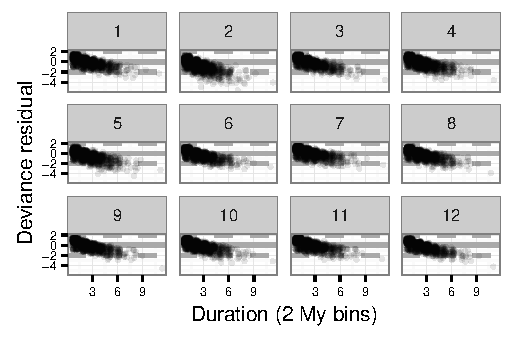
\includegraphics[height = 0.5\textheight, width = \textwidth, keepaspectratio = true]{figure/residual_plot}
  \caption{Deviance residuals from the fitted survival model compared to observed durations. Each graph depicts the residuals from single draws from the posterior distributions of all estimated parameters. Positive values indicate an underestimate of the observed duration, while negative values indicate an overestimate of the observed duration. A small amount of noise is added to each point to increase clarity. Twelve different examples are provided here to indicate consistency across multiple realizations.}
  \label{fig:ppc_res}
\end{figure}

\begin{figure}[ht]
  \centering
  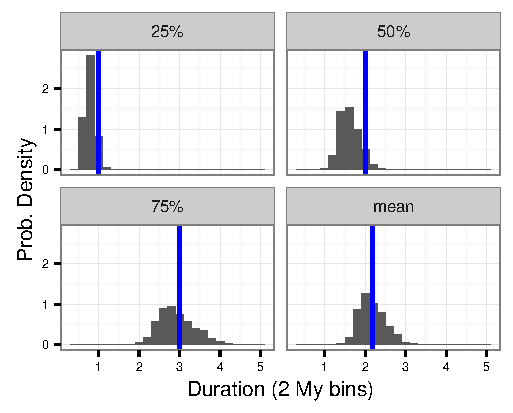
\includegraphics[height = 0.5\textheight, width = \textwidth, keepaspectratio = true]{figure/quant_ppc}
  \caption{The results of additional posterior predictive checks for four summaries of the observed durations, as labeled. Blue vertical lines indicate the observed value. None of the observed values are significantly different from the posterior predictive distributions.}
  \label{fig:ppc_quant}
\end{figure}

\begin{figure}[ht]
  \centering
  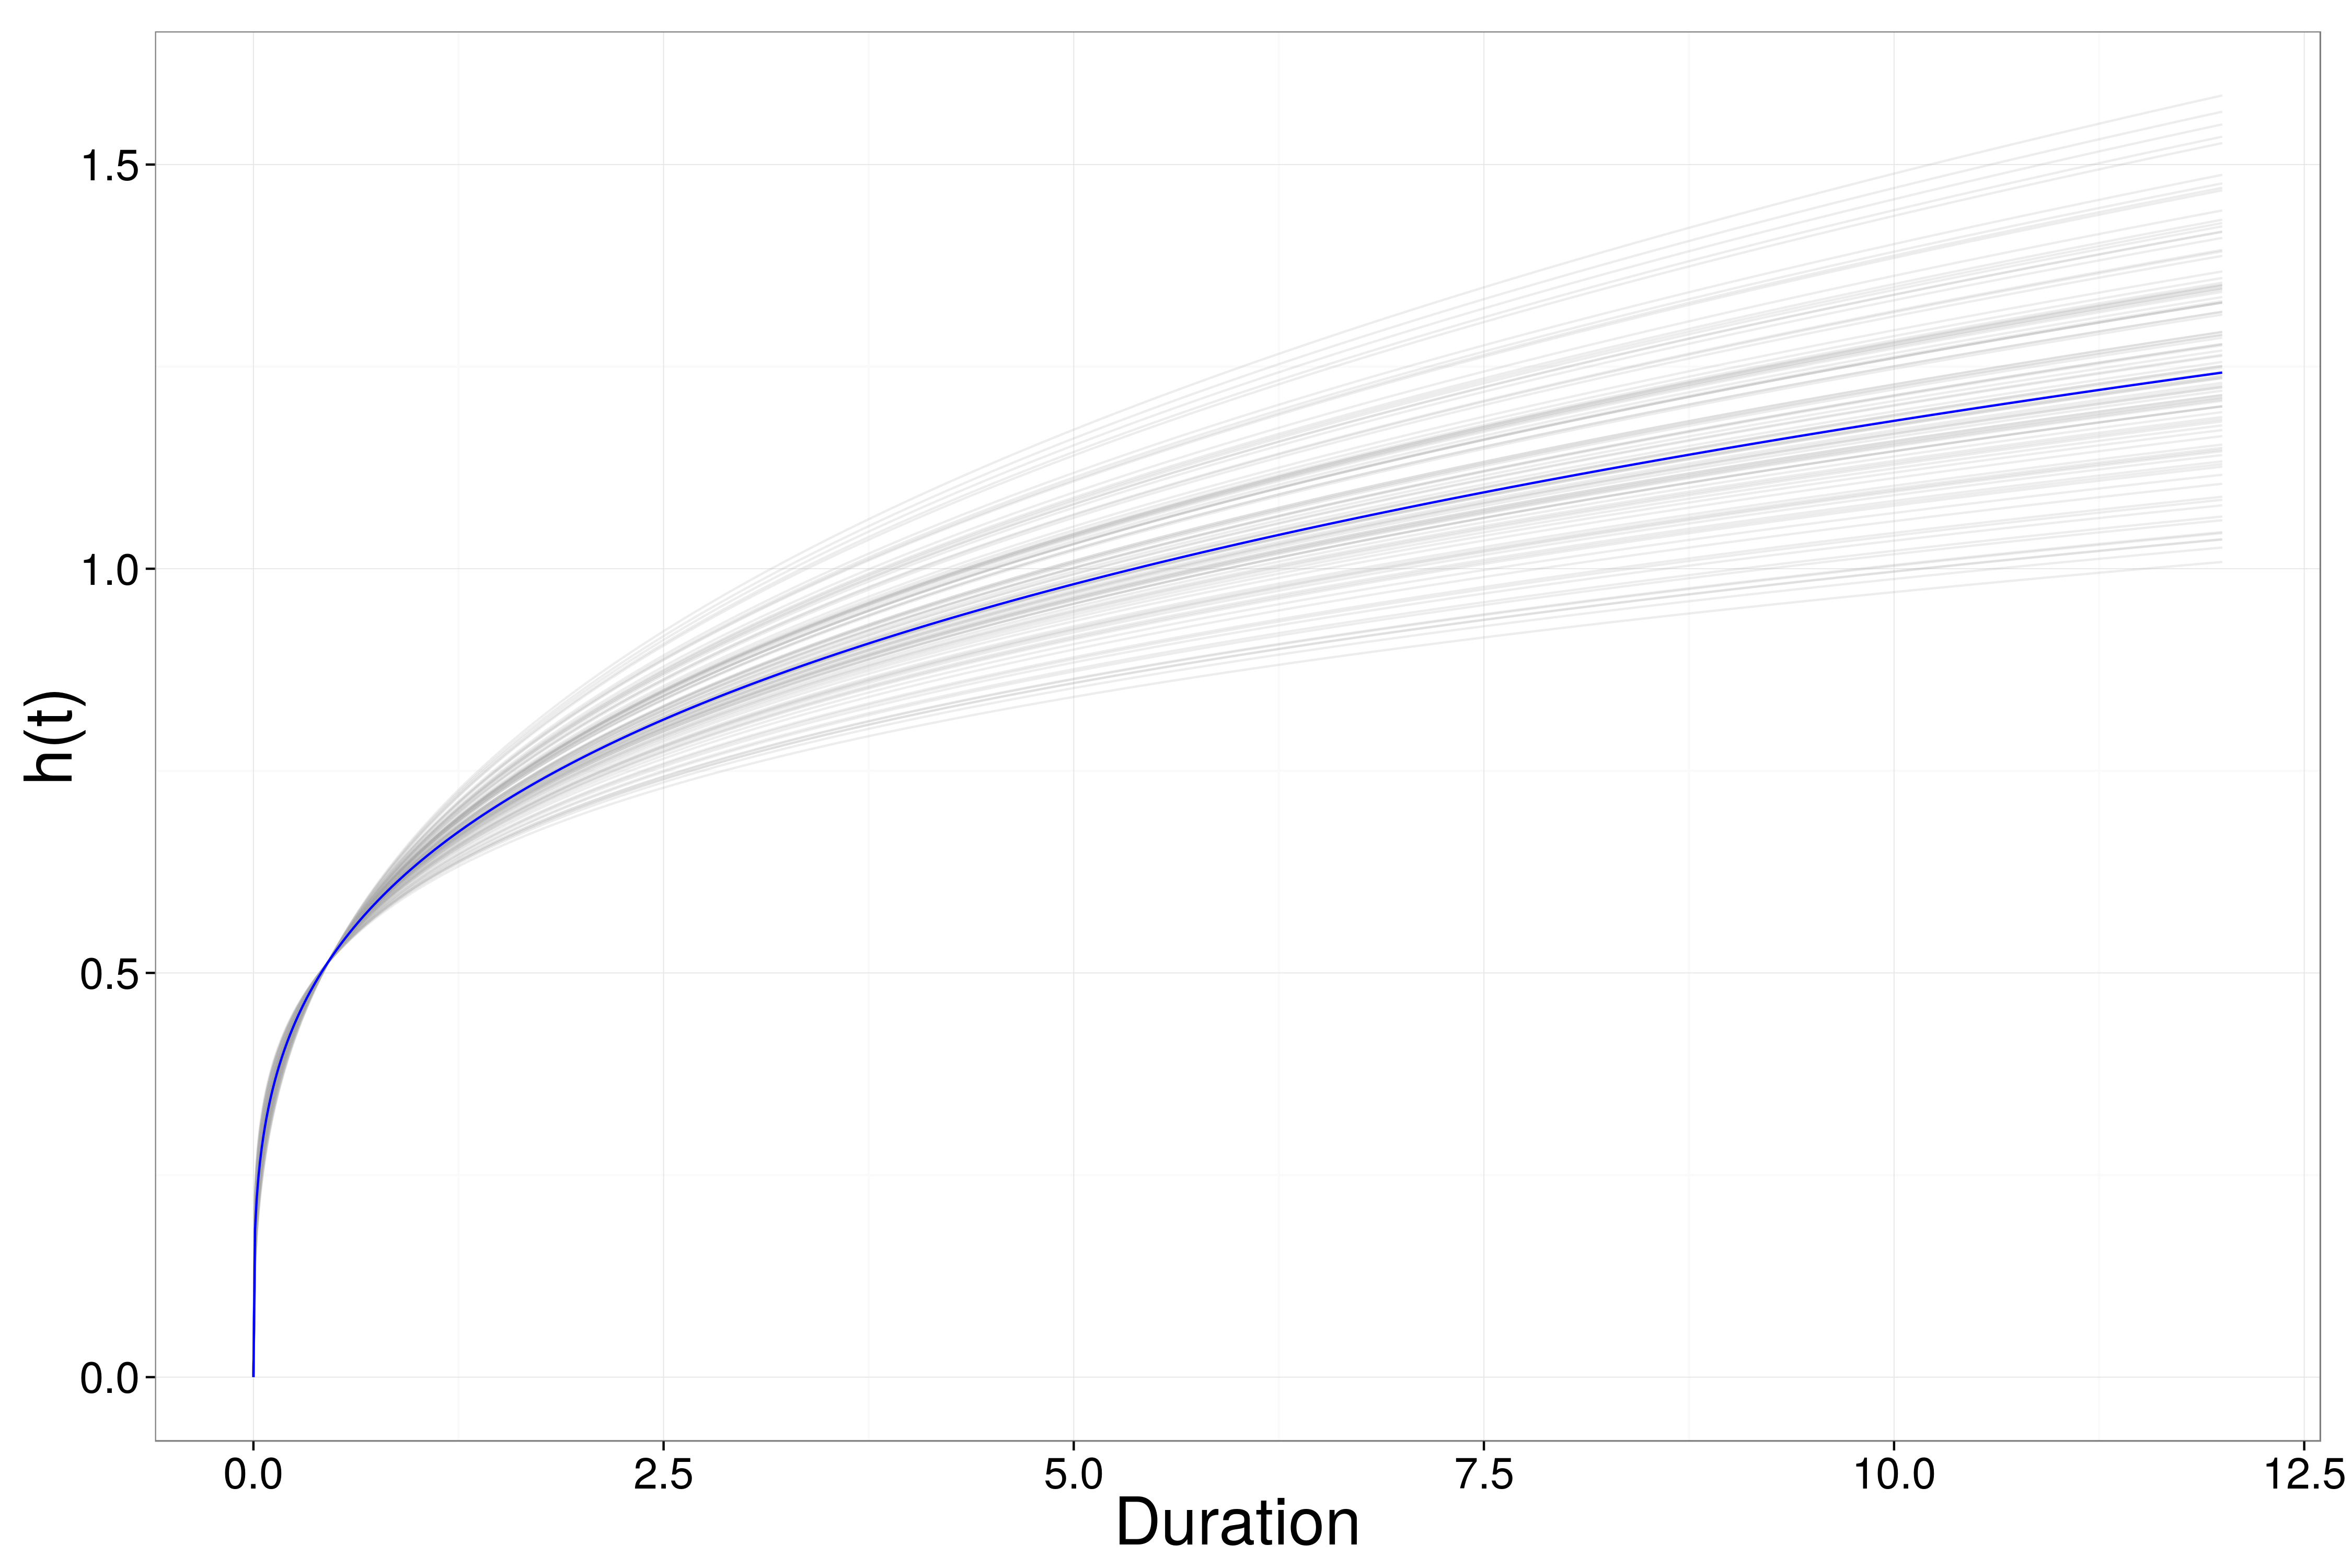
\includegraphics[height = 0.5\textheight, width = \textwidth, keepaspectratio = true]{figure/haz_est}
  \caption{1000 estimates of the hazard function (\(h(t\)) for the observed species mean (grey), along with the median estimated hazard function (blue). \(h(t)\) is an estimate of the rate at which a species of age \(t\) is expected to go extinct. Hazard functions were estimated from random draws from the estimated posterior distributions and evaluated with all covariate information set to 0, which corresponds to the expected duration of the mean species.}
  \label{fig:haz}
\end{figure}

\begin{figure}[ht]
  \centering
  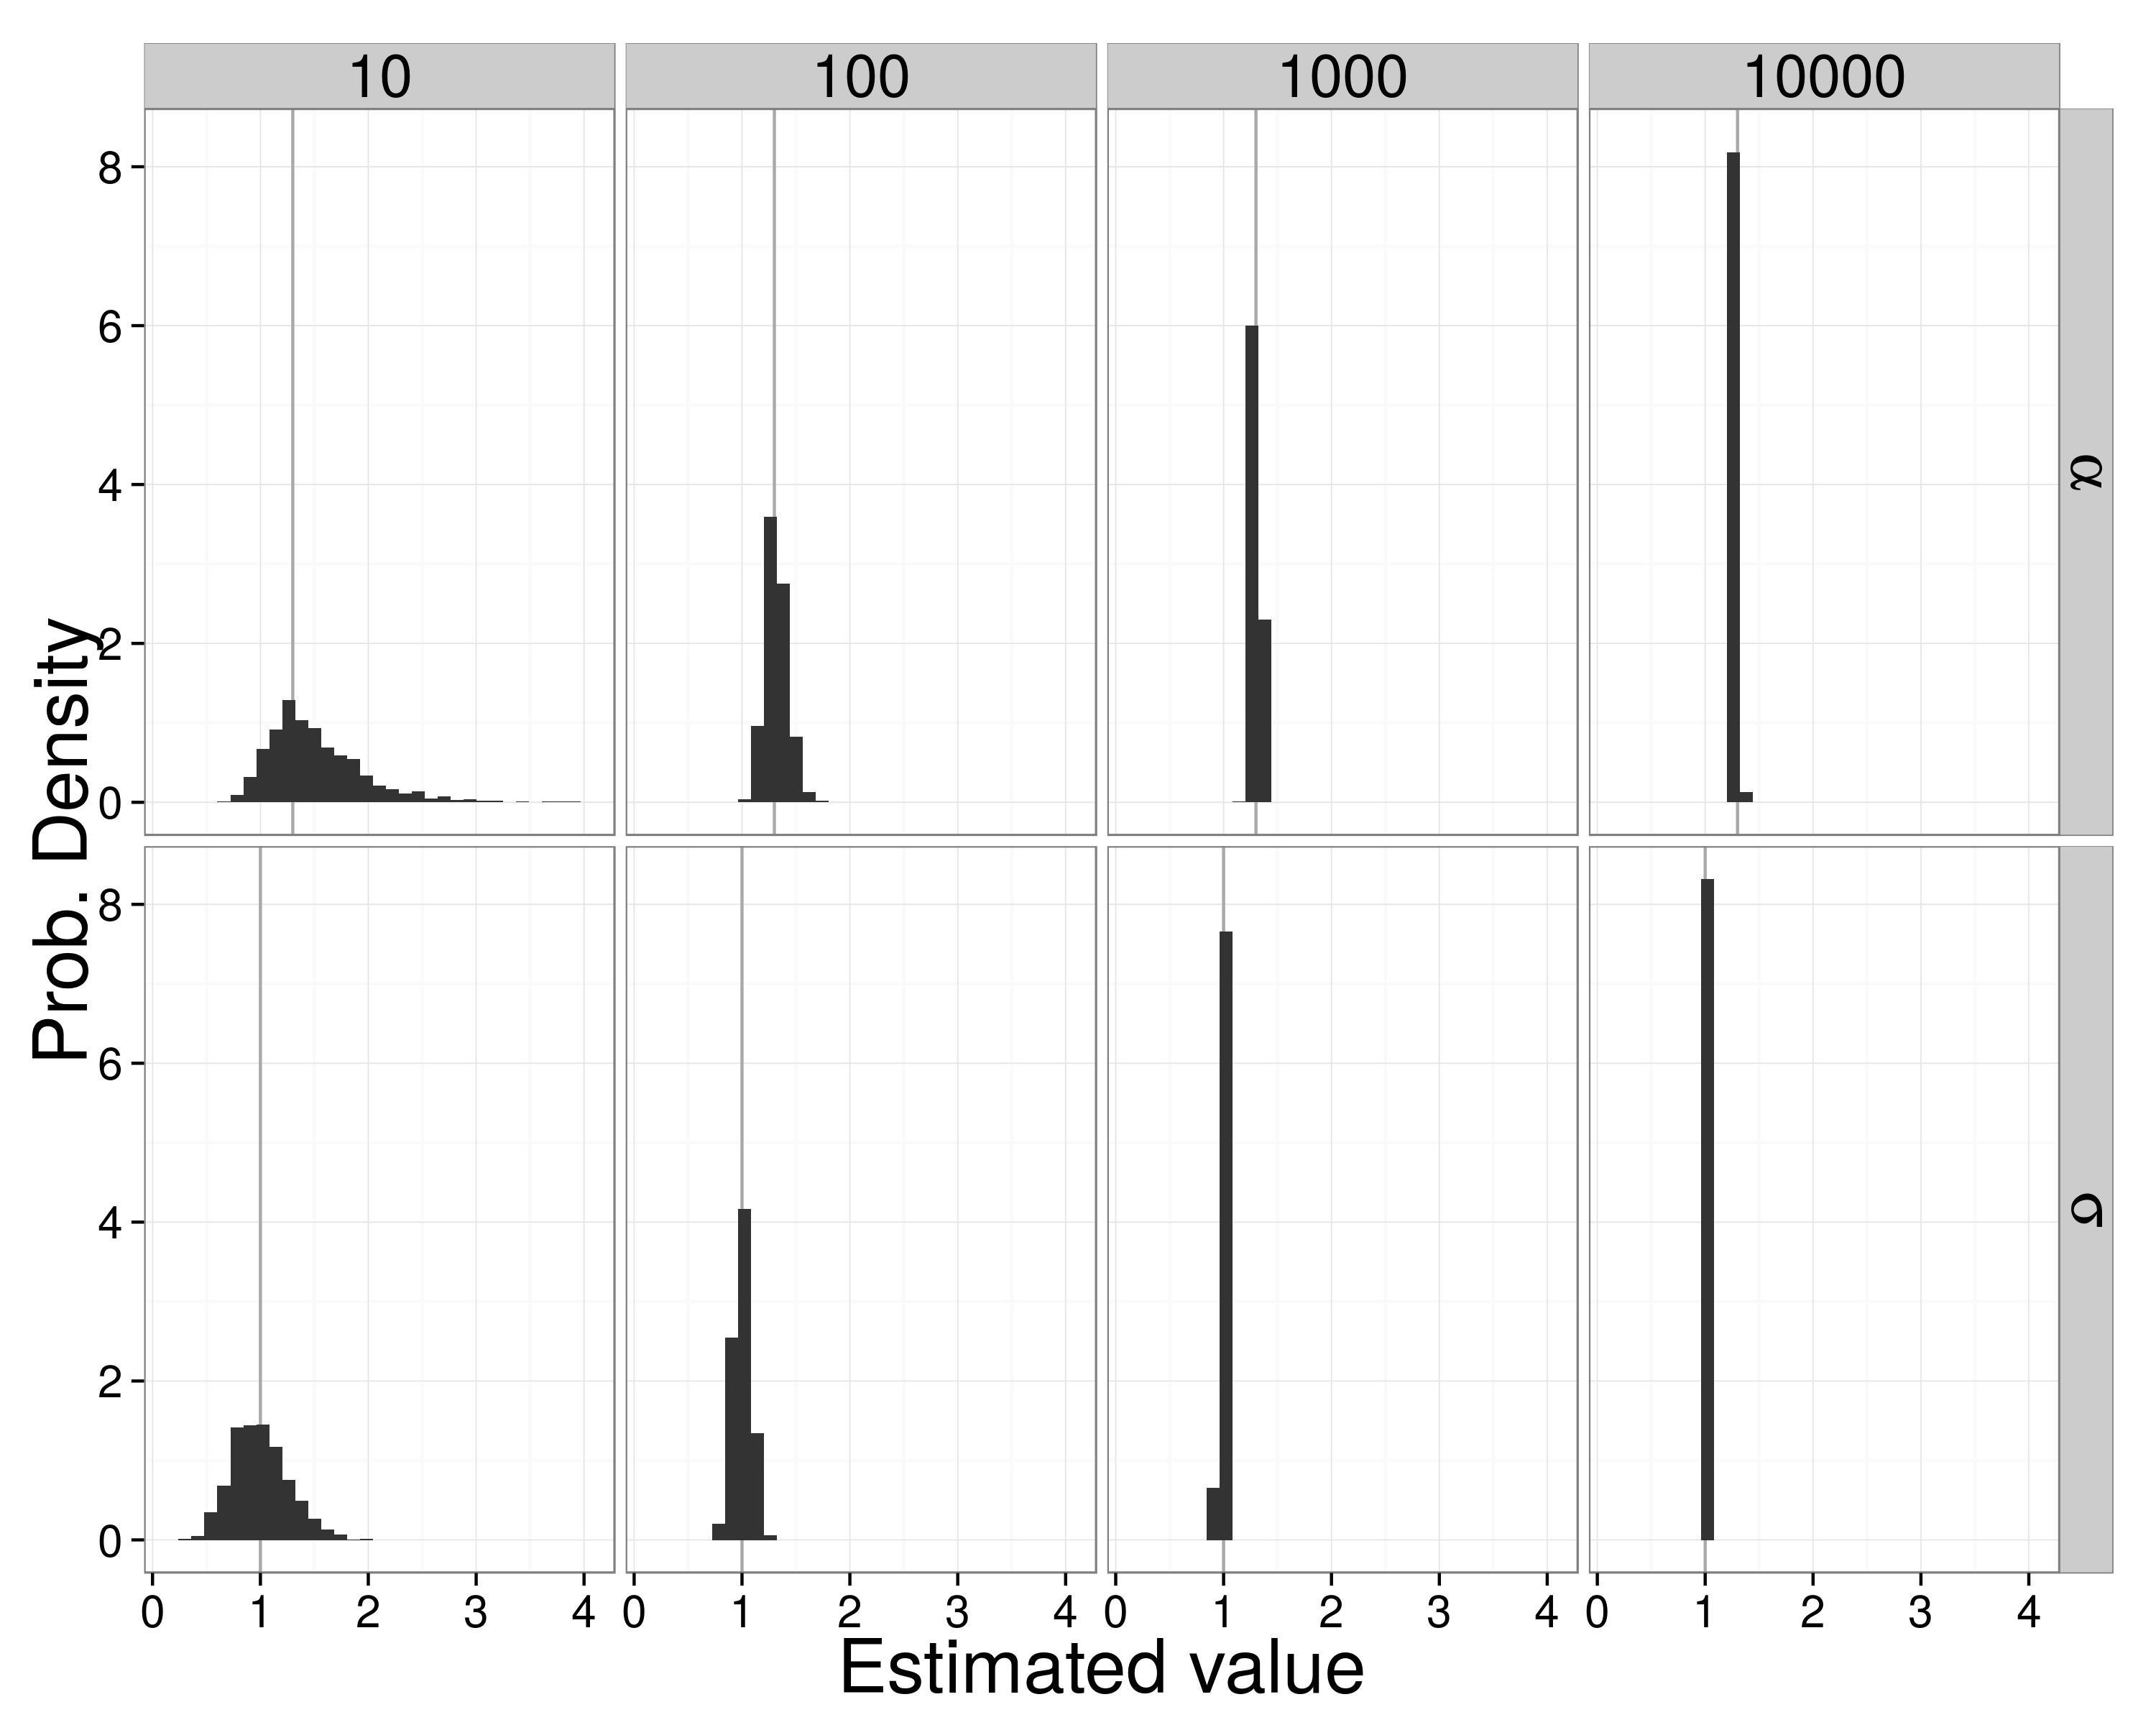
\includegraphics[height=0.5\textheight,width=\textwidth,keepaspectratio=true]{figure/alpha_simulation}
  \caption{Comparison of maximum likelihood estimates of shape (\(\alpha\)) and scale (\(\sigma\)) parameters from 1000 simulated data sets from 4 different sample sizes. Vertical lines are the actual parameter value used to generate the data. When sample size is approximately 100 or greater, estimates are not overly biased.}
  \label{fig:alpha_sims}
\end{figure}

\clearpage

\section{Supplementary tables}
\begin{table}[ht]
  \centering
  \caption{Species trait assignments in this study are a coarser version of the information available in the PBDB. Information was coarsened to improve per category sample size and uniformity and followed this table.}
  \begin{tabular}[ht]{ l | l | l }
    \hline
    \multicolumn{2}{ c |}{This study} & PBDB categories \\
    \hline \hline
    \multirow{4}{*}{Diet} & Carnivore & Carnivore \\
    & Herbivore & Browser, folivore, granivore, grazer, herbivore. \\
    & Insectivore & Insectivore. \\
    & Omnivore & Frugivore, omnivore. \\ 
    \hline
    \multirow{3}{*}{Locomotor} & Arboreal & Arboreal.\\
    & Ground dwelling & Fossorial, ground dwelling, semifossorial, saltatorial. \\
    & Scansorial & Scansorial. \\
    \hline
  \end{tabular}
  \label{tab:trait_cats}
\end{table}

\begin{table}[ht]
  \centering
  \caption{Regression equations used in this study for estimating body size. Equations are presented with reference to taxonomic grouping, part name, and reference.}
  \begin{tabular}{l | l | l | l}
    Group & Equation & log(Measurement) & Source \\
    \hline
    General & \(\log(m) = 1.827x + 1.81\) & lower m1 area &  \cite{Legendre1986} \\
    General & \(\log(m) = 2.9677x - 5.6712\) & mandible length & \cite{Foster2009a} \\
    General & \(\log(m) = 3.68x - 3.83\) & skull length & \cite{Luo2001} \\
    Carnivores & \(\log(m) = 2.97x + 1.681\) & lower m1 length & \cite{VanValkenburgh1990} \\
    Insectivores & \(\log(m) = 1.628x + 1.726\) & lower m1 area & \cite{Bloch1998} \\
    Insectivores & \(\log(m) = 1.714x + 0.886\) & upper M1 area & \cite{Bloch1998} \\
    Lagomorph & \(\log(m) = 2.671x - 2.671\) & lower toothrow area & \cite{Tomiya2013} \\
    Lagomorph & \(\log(m) = 4.468x - 3.002\) & lower m1 length & \cite{Tomiya2013} \\
    Marsupials & \(\log(m) = 3.284x + 1.83\) & upper M1 length & \cite{Gordon2003} \\
    Marsupials & \(\log(m) = 1.733x + 1.571\) & upper M1 area & \cite{Gordon2003} \\
    Rodentia & \(\log(m) = 1.767x + 2.172\) & lower m1 area & \cite{Legendre1986} \\
    Ungulates & \(\log(m) = 1.516x + 3.757\) & lower m1 area & \cite{Mendoza2006} \\
    Ungulates & \(\log(m) = 3.076x + 2.366\) & lower m2 length & \cite{Mendoza2006} \\
    Ungulates & \(\log(m) = 1.518x + 2.792\) & lower m2 area & \cite{Mendoza2006} \\
    Ungulates & \(\log(m) = 3.113x - 1.374\) & lower toothrow length & \cite{Mendoza2006} \\
    \hline
  \end{tabular}
  \label{tab:mass_est}
\end{table}

\clearpage 

\bibliographystyle{pnas}
\bibliography{newbib,packages}
\end{document}
